\documentclass[portrait,a1]{a0poster}
\usepackage{color,multicol}
\usepackage[english]{babel}
\usepackage[utf8]{inputenc}
\usepackage[T1]{fontenc}
\usepackage{siunitx}
\usepackage{graphicx}
\usepackage{booktabs}
\usepackage[round]{natbib}
\usepackage[font=small]{caption}
\usepackage{lmodern}
\usepackage[overload]{textcase}
\usepackage{setspace}
\usepackage{float}
\usepackage{lipsum} % Lorem ipsum generator

\columnsep = 50pt %change this for separation of the columns

\begin{document}

\definecolor{facultyColor}{cmyk}{0,.37,.88,.02} % faculty of science
\definecolor{gray}{cmyk}{.13,.05,0,.25}

%\vspace*{\fill} %some more marginal up

\begin{minipage}[t]{0.98\linewidth} % The first minipage for the logo & title
\vspace{0pt} % A trick to align the parallel minipages on top

%\vspace{0.008\linewidth} % Increase the top margin

\begin{minipage}[t]{0.48\linewidth} % logo
\vspace{0pt} % Alingns the parallel minipages on top
\includegraphics[width=0.4\linewidth]{HYlogo_fac_text-en}
\hspace{50pt}
\includegraphics[width=0.35\linewidth]{division}

\end{minipage} % no empty line before the next begin
\begin{minipage}[t]{0.5\linewidth} % title
\vspace{0pt} % Alingns the parallel minipages on top

\textsf{\bfseries
Jussi Tiira \\
Someone Else
} % Text size for a1 posters

\textcolor{gray}{\textsf{\bfseries{Department of Physics, Helsinki University}}}

\end{minipage}
\begin{minipage}[t]{1\linewidth}
\vspace{70pt}

\begin{spacing}{5.5}
% Highlight two first words of the title with the faculty color
{\Huge\usefont{T1}{phv}{bx}{n}\textcolor{facultyColor}{\MakeUppercase{Really long}} \MakeUppercase{and complex title for your poster}}
\end{spacing}

\end{minipage}
\end{minipage}

\vfill % some more marginal between header and text

\begin{multicols}{2} % change this for different number of columns

\section{Introduction}

Representation of precipitation, especially winter precipitation, in climate models is identified as one of the four most significant gaps in climate change studies \citep{schiermeier2010real}.

\lipsum[1]

\section{Methods}

\lipsum[2-3]

\begin{table}[H]
\centering
\begin{tabular}{ll}
\toprule
Instrument						& Measurements \\
\midrule
Ka Zenith radar (KAZR)			& Doppler spectra			\\
W-band radar (MWACR)				& Doppler spectra			\\
C-band dual-pol radar (IKA)		& $Z$, $K_{DP}$				\\
Microwave radiometer (MWR)		& LWP						\\
Particle Imaging Package (PIP)	& PSD, particle velocity		\\
Atmospheric sounding				& Thermodynamic state ($T$, $T_d$, $U$, $V$) \\
Pluviometer						& Precipitation accumulation	\\
Snow depth sensor				& Snow depth 				\\
\bottomrule
\end{tabular}
\caption{Instruments and measurements used for the study.}
\label{tab:instruments}
\end{table}

\section{Section}

\lipsum[4-5]

\begin{figure}[H]
  \centering
    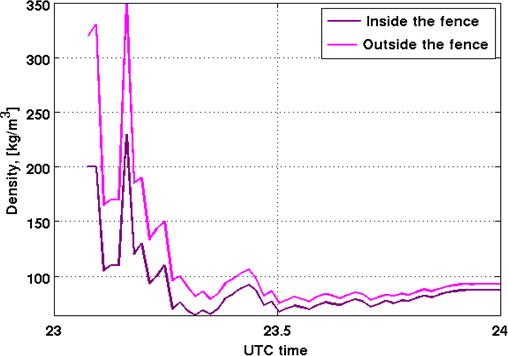
\includegraphics[width=0.7\columnwidth]{density}
  \caption{Snow density in \si{\kilo\g\per\cubic\metre} calculated using pluviometers located inside and outside the fence between 23:00 UTC and 24:00 UTC.}
  \label{fig:sounding}
\end{figure}

\section{Conclusions}

\begin{itemize}
\item \lipsum[6]
\item \lipsum[7]
\end{itemize}

\bibliographystyle{abbrvnat}
\bibliography{ref}

\end{multicols}

\vfill %some more marginal in the end

\end{document}